% Déclaration du type de document (report, book, paper, etc...)
\documentclass[a4paper]{paper} 
 
% Package pour avoir Latex en français
\usepackage[utf8]{inputenc}
\usepackage[T1]{fontenc}
\usepackage[frenchb]{babel}
 
% Quelques packages utiles
\usepackage{listings} % Pour afficher des listings de programmes
\usepackage{graphicx} % Pour afficher des figures
\usepackage{amsthm}   % Pour créer des théorèmes et des définitions
\usepackage{amsmath}
\usepackage{microtype} % Optical margins FTW
\usepackage{url}
\usepackage{booktabs} % Allows the use of \toprule, \midrule and \bottomrule in tables for horizontal lines
\usepackage[per-mode=symbol]{siunitx}
\usepackage{floatrow}
\usepackage{caption}
\usepackage{subcaption}
\usepackage{mhchem}

% Unités customs pour les francs et les pièces
\DeclareSIUnit\chf{\textsc{chf}}
\DeclareSIUnit\piece{pièce}
\DeclareSIUnit\annee{année}
\DeclareSIUnit\an{an}



% Début du document
\begin{document}

\begin{titlepage}

\newcommand{\HRule}{\rule{\linewidth}{0.5mm}} % Defines a new command for the horizontal lines, change thickness here

\center % Center everything on the page 
%----------------------------------------------------------------------------------------
%	HEADING 
%----------------------------------------------------------------------------------------
\textsc{\LARGE École Polytechnique Fédérale de~Lausanne}\\[1.5cm] 
\textsc{\Large Méthodes de Production}\\[0.5cm] % Major heading such as course name

%----------------------------------------------------------------------------------------
%	TITLE 
%----------------------------------------------------------------------------------------
\HRule \\[0.4cm]
{ \huge \bfseries Molded Interconnect Devices}\\[0.4cm] % Title of your document
\HRule \\[1.5cm]
 
%----------------------------------------------------------------------------------------
% LOGO EPFL
%----------------------------------------------------------------------------------------
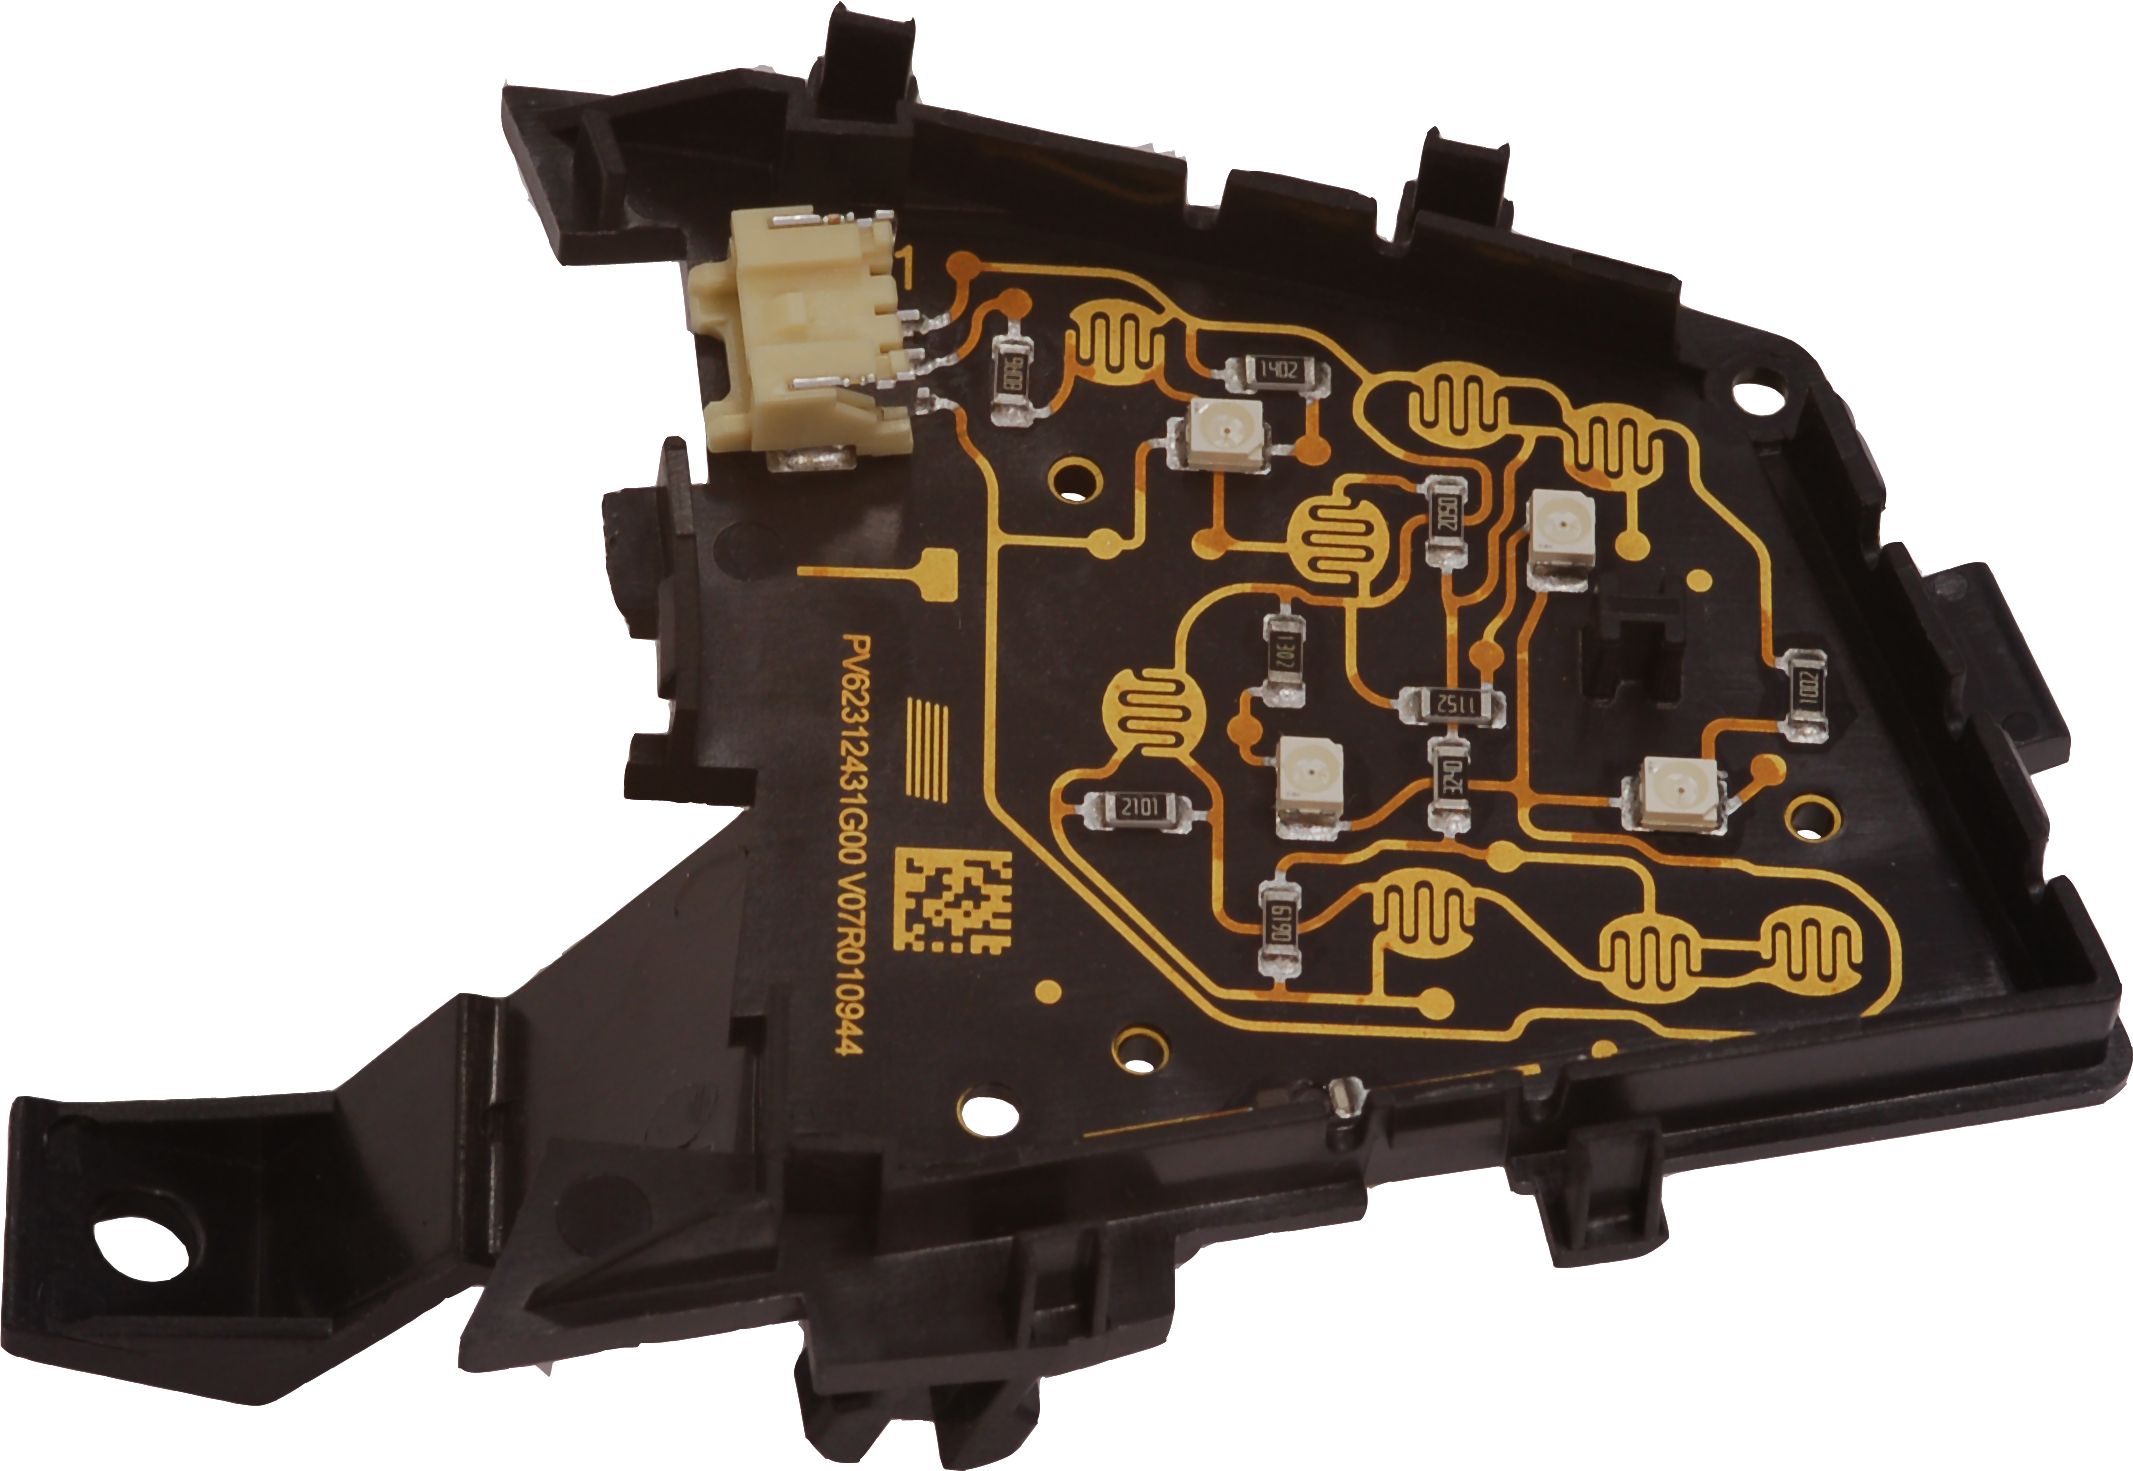
\includegraphics[width=0.8\textwidth]{../images/mid_example}\\[2cm]

%----------------------------------------------------------------------------------------
%	AUTHORS 
%----------------------------------------------------------------------------------------

\vfill % Fill the rest of the page with whitespace
\begin{minipage}{0.55\textwidth}
\begin{flushleft} \large
\emph{Étudiants:}\\
Antoine \textsc{Albertelli}\\ 
Quentin \textsc{Herzig}
\end{flushleft}
\end{minipage}
~
\begin{minipage}{0.4\textwidth}
\begin{flushleft} \large
\emph{Enseignants:} \\
Pr. Jacques \textsc{Jacot} \\
Pr. Peter \textsc{Ryser}\\
Dr. Jean-Daniel \textsc{Lüthi}
\end{flushleft}
\end{minipage}\\[2cm]


{\large 13 décembre 2013}
\end{titlepage}

% Empty page after title page.
\begin{titlepage}
    ~
\end{titlepage}



\tableofcontents

\section{Introduction}
Un \gls{mid}  est un circuit électronique
dont le support est un substrat thermoplastique moulé par injection, par
opposition au \textsc{PCB} conventionnels dont le substrat est un composite
plat.

Les \gls{mid} permettent de regrouper dans une seule pièce des fonctions
mécaniques et éléctroniques. En effet, contrairement au \textsc{pcb} conventionnels, les
\gls{mid} peuvent être conçus en trois dimensions, ce qui réduit
considérablement le nombre de composants et de connecteurs, diminuant ainsi le
temps d'assemblage, et donc le coût du système. 

Les \gls{mid}s ne sont toutefois pas une solution de remplacement des
\textsc{pcb}s car ils ne permettent pas une grande densité de pistes, tandis que
les \textsc{pcb}s à plus de deux couches sont désormais peu coûteux et
permettent des circuits à forte densité.


\section{Conception de MID}
La conception des \gls{mid} commence par la création du schéma électrique dans un logiciel de conception électronique standard, puis le schéma est exporté sous forme de \emph{netlist}, c'est à dire d'une liste de connexion entre différents composants.
Le design mécanique du \gls{mid} se fait dans un logiciel de \textsc{dao} standard, comme Solidworks puis est exporté au format \textsc{step}.

La \emph{netlist} et le fichier \textsc{step} sont ensuite importés dans un logiciel spécifique \footnote{Nextra de chez Mecadtron \url{http://www.mecadtron.com/produkte/nextra.en.php}} pour l'étape de routage (placement des pistes).
Lors de cette étape on place aussi des repères appelés \emph{fiducials} qui seront utilisés par les machines d'activation et d'assemblage pour faire un alignement visuel.
On peut également placer des codes-barres 2D (\emph{datamatrix}) qui seront modifiés par la machine d'activation pour y placer un numéro de série, afin de faire du suivi des pièces.

\subsection{Matériaux utilisables}
Les contraintes inhérentes à la technologie \gls{lds} limitent fortement le choix des matériaux :
\begin{itemize}
    \item La pièce étant injectée puis activée, le matériaux choisi doit être un thermoplastique,
    \item Pour l'étape d'activation, le polymère doit pouvoir se lier avec un dopant organométallique, généralement à base de palladium,
    \item L'assemblage des composants par \textit{reflow soldering} exige une température de fusion élevée.
\end{itemize}

LPKF a donc créé une liste de matériaux utilisables et reccomandés pour le \gls{lds}.
Cette liste est visible dans le tab. \ref{tab:mid-materials}.
Une liste de fournisseur proposant ces matériaux déjà dopés est également disponible chez LPKF \cite{mid-design-rules}.

% Table des matériaux
\begin{table}[h]
\centering
\begin{tabular}{l l}
\toprule 
Type & Matériau \\
\midrule % In-table horizontal line
LCP & Liquid Crystal Polymer \\
PA 6/6T & Polyamide \\
PBT & Polytéréphtalate de butylène \\
PBT/PET & Mélange de PBT et de PET \\
PPA & Polyphthalamide \\
PC & Polycarbonate \\
PC/ABS & Mélange de PC et d'ABS \\ 
\bottomrule 
\end{tabular}
\caption{Matériaux utilisables comme substrat}
\label{tab:mid-materials}
\floatfoot{Source: \cite{mid-design-rules}}
\end{table}

\subsection{Limites du procédé LDS}
La conception de circuits \gls{mid} est délicate car elle doit prendre en compte des limites provenant de l'injection plastique, de l'activation laser et de la métallisation.
L'ingénieur doit donc porter une attention particulière aux détails lors de la conception, car des petits détails, comme des trous borgnes, peuvent augmenter significativement le coût de la pièce, voir même la rendre impossible à réaliser.
L'ensemble des règles de conception à respecter est compilée dans un seul document, fourni par LPKF \cite{mid-design-rules}.
Nous allons ici nous concentrer sur les plus importantes.

La plus grosse limitation des \gls{mid} par rapport au \gls{pcb} est la faible densité de pistes atteignable.
En effet, il est impossible de fabriquer des \gls{mid} avec des couches internes, là où des circuits à 16 couches sont facilement atteignables dans le domaine des \gls{pcb}.
De plus, les \glspl{mid} ne permettent pas de faire des pistes très fines ou très serrées : On considére généralement qu'il faut rester au dessus de \SI{150}{\micro\meter} .

\textbf{A compléter\ldots}



\section{Procédés de fabrication des MID}
Il existe actuellement 2 méthodes de production de \gls{mid} sur le marché : le \gls{lds} et le \emph{Two-shot molding}.
Depuis son introduction sur le marché en 2006, le \gls{lds} a pratiquement éclipsé le Two-shot, car celui ci est plus compliqué à mettre en oeuvre et plus cher.
Le two-shot était surtout utilisé pour produire des grandes quantités à bas coût mais avec la baisse des prix, le \gls{lds} est désormais utilisé pour la production de masse.
Par exemple, Molex, le plus gros constructeur d'antennes \textsc{smd} au monde utilise actuellement uniquement le procédé \gls{lds}.

\subsection{Laser Direct Structuring}
\begin{figure}[h]
    \begin{center}
        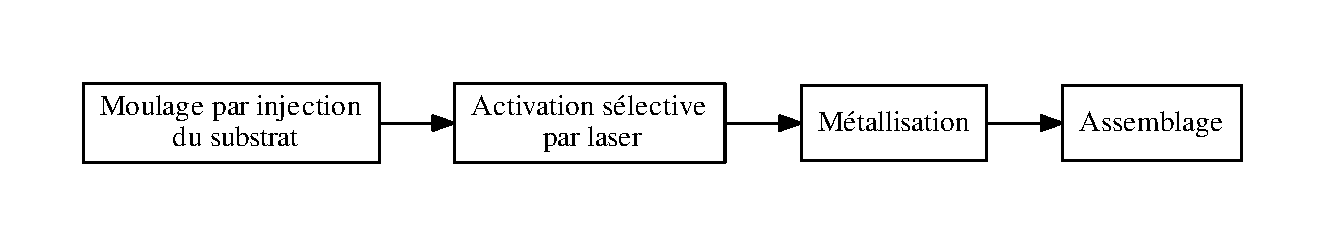
\includegraphics[width=\textwidth]{images/lds_process}
        \caption{Vue d'ensemble du processus \emph{Laser Direct Structuring}}\label{fig:lds-process}
    \end{center}
\end{figure}
Le \gls{lds} est un procédé relativement récent, ayant été introduit sur le marché en 2006.
Par conséquent, c'est une technologie brevetée de LPKF~Lasers~\&~Electronics~AG en Allemagne.
Leur site web\footnote{\url{www.lpkf.com}} est donc une excellente source d'informations pour la conception de pièces utilisant le \gls{lds}.

\subsubsection{Principe de base du procédé}
Le principe général du procédé est visible à la fig.
\ref{fig:lds-process}.
On retrouve donc, dans l'ordre :

\begin{description}
    \item[Injection] La pièce esLa pièce est d'abord moulée par un procédé d'injection standard.
        Le détail de cette étape sort du cadre de ce séminaire.
        On se référera à celui sur l'injection plastique.

    \item[Activation] Le polymère ayant servi pour l'injection de la pièce a préalablement été dopé avec un composant organométallique qui est activé par le laser en suivant le tracé des pistes voulues.
        Une réaction physique décompose alors ce dopant entre partie métallique et partie organique.
    Les lasers utilisés sont typiquement des lasers infra-rouges d'une \item[Métallisation] L'étape de métallisation commence par une étape de nettoyage, afin de faciliter l'accrochage.
        Les pistes sont ensuites construites par dépose de fine couches (environ \SI{5}{\micro\meter}).
        Finalement, un traitement de surface contre l'oxydation est appliqué.
        Ce traitement consiste généralement en une couche de nickel suivi d'une couche d'or, mais des traitements spécifiques, à base d'étain ou d'argent sont également possibles.
    \item[Assemblage] Les composants électriques annexes (boutons, connecteurs, etc\ldots) sont soudés sur le \gls{mid}.
        Pendant le prototypage cette étape est souvent faite à la main, avec un fer à souder.
        Pour la production, si le polymère a une température de fusion suffisament élevée, l'assemblage par \emph{reflow soldering} est possible.

\end{description}

\subsubsection{Métallisation}
L'étape de métallisation est celle qui va déposer les pistes sur le poylmére à proprement parler.
Afin de garantir le bon fonctionnement de cette étape, un rinçage de la pièce entre chaque bains est effectué, ainsi qu'un séchage à chaud après le dernier bain, afin d'enlever toute trace sur la pièce finale.

Le premier bain de cuivre se fait sans électrolyse, vu qu'aucune piste conductrice n'existe pour le moment.
Dans ce bain, du cuivre va croître autour des atomes de métail présent à la surface du polymère et se liera au microcavités résultant de l'activation laser.
L'épaisseur maximum atteignable lors de ce premier bain est de 5 à 8 \si{\micro\meter}.

Dans les applications à fort courants, une grande épaisseur de cuivre est souhaitée.
Pour y parvernir, on peut, après le premier bain, faire une dépose éléctrolytique du cuivre.
Pour cela, il faut que toute les pistes soit connectées entre elles en un point.
Si ce n'était pas le cas, il faudrait connecter les pistes une à une à l'éléctrode, ce qui serait long et donc coûteux.
Le point de connexion est généralement placé sur une partie séparable mécaniquement qui est enlevée après la métallisation.

Une fois ce premier bain terminé, une couche de protection contre l'oxydation est appliquée.
En effet une oxydation de la couche de cuivre ruinerait les proprietés électriques du circuit.
Cette couche est généralement composée d'une couche de nickel suivie d'une couche d'or.
Le rôle de cette dernière est d'empêcher l'oxydation de la couche de cuivre, tandis que la couche de nickel sert à empêcher le cuivre de diffuser dans l'or, ce qui détruirait la protection anti-oxydation.
Avant le traitement anti-oxydant, la pièce est passée dans un bain de palladium \footnote{\emph{A vérifier :} \ce{PdCl2}} afin de catalyser la dépose du nickel.

\subsection{Two-shot molding}
Le two-shot molding est un procédé antérieur au \gls{lds} et qui n'est pas breveté.
Il est essentiellement utilisé dans le milieu de l'injection plastique, pour produire des pièces injectées de différentes couleurs, comme des touches de clavier d'ordinateur.
Cette méthode consiste à d'abord mouler les pistes dans un polymère dopé, puis à ``surmouler'' la forme définitive de la pièce autour (fig. \ref{fig:second-shot}).
Finalement, la pièce est métalisée suivant le même procédé que dans le \gls{lds}, mais le cuivre ne se dépose que sur les parties exposées du polymère dopé (fig. \ref{fig:two-shot-metal}).


\begin{figure}[h]
        \centering
        \begin{subfigure}[t]{0.3\textwidth}
                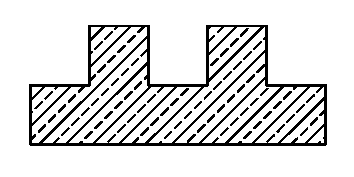
\includegraphics[width=\textwidth]{images/two-shot-example/inner}
                \caption{Injection du polymère dopé.}
                \label{fig:first-shot}
        \end{subfigure}%
        ~ 
        \begin{subfigure}[t]{0.3\textwidth}
                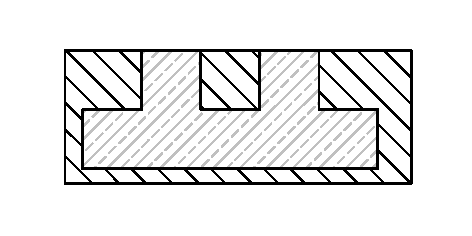
\includegraphics[width=\textwidth]{images/two-shot-example/second_shot}
                \caption{Surmoulage d'un polymère standard.}
                \label{fig:second-shot}
        \end{subfigure}
        ~
        \begin{subfigure}[t]{0.3\textwidth}
                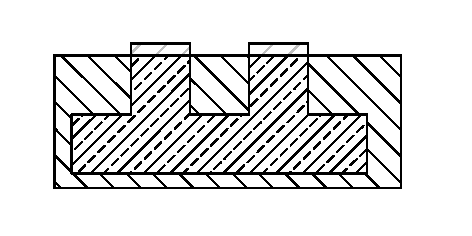
\includegraphics[width=\textwidth]{images/two-shot-example/after_metal}
                \caption{Métallisation.}
                \label{fig:two-shot-metal}
        \end{subfigure}
        \caption{Procédé two-shot}\label{fig:two-shot-process}
\end{figure}



\section{Étude de coûts}

\begin{figure}[h]
        \centering
        \begin{subfigure}[t]{0.4\textwidth}
            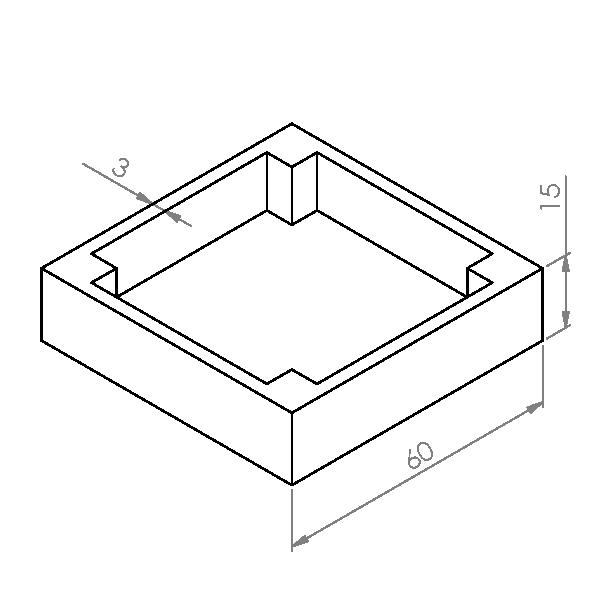
\includegraphics[width=\textwidth]{images/example_part/example_mid}
            \caption{Partie mécanique. Dimensions en \si{\milli\meter}.}
        \end{subfigure}
        ~
        \begin{subfigure}[t]{0.4\textwidth}
                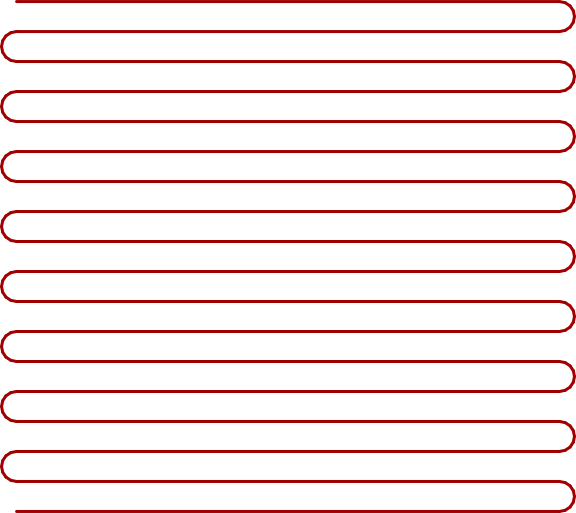
\includegraphics[width=\textwidth]{images/example_part/tracks.png}
                \caption{Tracé des pistes (similaire pour les cinq faces intérieures).}
        \end{subfigure}

        \caption{Pièce d'exemple. Les dimensions et la géométrie sont approximatives. La largeur des pistes et la distance entre deux pistes est de \SI{150}{\micro\meter}.}
        \label{fig:example-part}
\end{figure}
Pour notre étude de coûts, nous avons décidé de nous baser sur la série en production chez Cicorel lors de notre visite.
Les tableaux de calculs de coûts restent néanmoins valables, moyennant un changement de certaines valeurs.
Les paramètres à changer en fonction de la pièce sont indiqués dans le détail de chaque partie.


\paragraph{Descriptif de la pièce}
La pièce que nous considérons est une pièce relativement simple.
Il s'agit d'un couvercle anti-ingénierie inverse pour lecteur de carte de crédit.
Le rôle de cette pièce est de détecter toute tentative d'accéder à l'intérieur de l'appareil, soit en le démontant, soit en le perçant.
Pour accomplir cette fonction, deux pistes sont placées en serpentin à l'intérieur du couvercle.
L'appareil est programmé pour effacer toute les données sensibles dès qu'une de ces pistes est rompue.
Cette pièce était malheureusement confidentielle et nous n'avons pas pu la prendre en photo.
On peut l'approximer par la boîte creuse visible à la fig. \ref{fig:example-part}.


\subsection{Injection}
\begin{table}[h!]
\centering 
\begin{tabular}{l S[table-format=3.2] r} 
\toprule 
\multicolumn{2}{l}{\textbf{Électricité}} & \\ 
Consommation électrique & 5 & \si{\kilo\watt} \\
Prix de l'électricité & 0.2 & \si{\chf\per\kilo\watt\per\hour} \\
\cmidrule(l){2-3}
Coût d'électricité & 1 & \si{\chf\per\hour} \\
\midrule
\multicolumn{2}{l}{\textbf{Machines}} & \\ 
Presse électrique & 130000 & \si{\chf} \\
Fonctionnement & 6240 & \si{\hour\per\annee} \\
\cmidrule(l){2-3}
Amortissement sur 5 ans & 4.17 & \si{\chf\per\hour} \\
\midrule
\multicolumn{2}{l}{\textbf{Opérateurs}} & \\ 
Opérateur à 10\% & 6& \si{\chf\per\hour} \\
\midrule

\multicolumn{2}{l}{\textbf{Matière}} & \\ 
Matière (\textsc{pc}) & 11 & \si{\chf\per\kilogram} \\ 
Poids de la pièce & 25 & \si{\gram} \\
\cmidrule(l){2-3}
Coût de la matière & 0.27 & \si{\chf\per\piece} \\

\midrule
\multicolumn{2}{l}{\textbf{Outillage}} & \\ 
Prix du moule & 20000 & \si{\chf} \\
Pièces par série & 20000& \si{\piece} \\
\cmidrule(l){2-3}
Coûts d'outillage & 1 & \si{\chf\per\piece} \\

\midrule
\midrule
Coût horaire & 11.67  & \si{\chf\per\hour} \\
Temps de cycle & 20 & \si{\second\per\piece} \\
\cmidrule(l){2-3}
\textbf{\textsc{Total}} & 1.34 & \si{\chf\per\piece} \\

\bottomrule 
\end{tabular}
\caption{Calcul des coûts de l'injection plastique} 
\label{tab:cost-molding}
\end{table}



L'étape d'injection plastique demande un moule usiné soit par éléctroérosion, soit par usinage à grande vitesse.
Le coût du moule a été estimé suivant les calculs présentés dans le séminaire\cite{electroerosion-2013}.
Le détail de ces calculs sortant du cadre du présent séminaire, nous avons fait le choix de ne pas les inclure. 

Nous avons également supposé que la pièce est faite dans la matière la moins cher, c'est à dire le polycarbonate.
Les polymères activables sont environ 20\% plus cher que leur homologue non activable d'après notre contact chez Cicorel.
Les prix des matériaux varient entre \SI{11}{\chf\per\kilogram} pour du \textsc{pc} et \SI{220}{\chf\per\kilogram} pour du \textsc{peek}.

\subsection{Activation Laser}
Pour calculer le coût de l'étape d'activation sélective (\gls{lds}) nous avons fait quelques hypothèses :
\begin{itemize}
    \item Le secteur d'activation laser tourne \SI{24}{\hour} par jour, 5 jours sur 7.
    \item La machine est une Microline 160i de chez LPKF coûtant \SI{220000}{\chf}.
        Elle est amortie en 5 ans.
    \item Un opérateur ne peut s'occuper que d'une machine à la fois.
    \item La machine consomme en permanence sa puissance de pointe soit \SI{2.5}{\kilo\watt} \cite{lpkf-microline-series}.
        L'électricité représentant une fraction faible du coût final, cette hypothèse n'induis pas de grande erreurs.
\end{itemize}

Le calcul de la surface occuppée par les pistes sur notre circuit se base sur une largeur de piste de \SI{150}{\micro\meter} et une
distance entre deux pistes de \SI{150}{\micro\meter} également, pour une piste occupant toute la surface du circuit.
Pour une autre pièce, la surface des pistes peut souvent être obtenue dans le logiciel de conception.

\begin{table}[h!]
\centering 
\begin{tabular}{l S[table-format=3.2] r} 
\toprule 
\multicolumn{2}{l}{\textbf{Électricité}} & \\ 
Consommation électrique & 2.5 & \si{\kilo\watt} \\
Prix de l'électricité & 0.2 & \si{\chf\per\kilo\watt\per\hour} \\
\cmidrule(l){2-3}
Prix de l'électricité & 0.5 & \si{\chf\per\hour} \\
\midrule
\multicolumn{2}{l}{\textbf{Machines}} & \\ 
LPKF Microline 160i & 220000 & \si{\chf} \\
Fonctionnement & 6240 & \si{\hour\per\annee} \\
\cmidrule(l){2-3}
Amortissement sur 5 ans& 7.05 & \si{\chf\per\hour} \\
\midrule
\multicolumn{2}{l}{\textbf{Opérateurs}} & \\ 
Opérateur à 100\% & 60& \si{\chf\per\hour} \\

\midrule
\multicolumn{2}{l}{\textbf{Temps de cycle}} & \\ 
Vitesse du laser & 4000 & \si{\milli\meter\per\second} \\
Diamètre du laser & 80 & \si{\micro\meter} \\
Vitesse de balayage & 320 & \si{\milli\meter\squared\per\second} \\
Surface des pistes & 1800 & \si{\milli\meter\squared\per\piece} \\ 
Temps de balayage & 5.625 & \si{\second\per\piece} \\ 
Temps de positionnement & 1 & \si{\second\per orientation} \\
Nombre d'orientations & 5 &  \\
Temps de mise en place, retrait et inspection & 15 & \si{\second\per\piece} \\ 

\cmidrule(l){2-3}
\textbf{Temps total} & 25.625 & \si{\second\per\piece} \\ 

\midrule
\midrule
Coût horaire & 67.68 & \si{\chf\per\hour} \\
Temps de cycle & 25.625 & \si{\second\per\piece} \\
\cmidrule(l){2-3}
\textbf{\textsc{Total}} & 0.48 & \si{\chf\per\piece} \\

\bottomrule 
\end{tabular}
\caption{Calcul des coûts de l'activation sélective par laser} 
\label{tab:cost-laser-activation}
\end{table}


\subsection{Métallisation}
Calculer le coût réel de cette étape est difficile, car beaucoup d'informations ne sont pas disponibles publiquement : le prix des bains et de la \gls{step} pour ne citer que ces deux là, ne sont pas trouvable chez les fournisseurs.
De plus, filtrer les bains pour les recycler permet de récupérer un peu de matière qui est revendue, ce qui intervient dans le calcul de coût, mais est difficile à estimer.
Finalement, notre contact chez Cicorel a refusé de détailler leur méthode de calculs pour ces bains, en nous répondant qu'il s'agissait de données internes et confidentielles.

Nous avons donc estimé que le coût pour déposer \SI{1}{\kilogram} de métal par voie chimique était environ cinq fois le prix de ce métal sur le marché.
Ce coût inclut la \gls{step}, le chauffage des bains et l'électricité consommée par le robot servant à déplacer les pièces d'un bain au suivant. 
Cette estimation peut sembler hasardeuse, mais elle donne néanmoins une approximation suffisante pour l'ingénieur désireux d'utiliser ce procédé.
À ce coût des matériaux, il faut ajouter l'amortissement de la machine sur cinq ans et l'opérateur (deux opérateur pour trois lignes).

Pour estimer le temps de cycle, nous avons le temps de l'étape la plus longue, c'est à dire la déposition du cuivre.
En effet, une fois un rack sorti du bain de cuivre, un autre peut prendre sa place tandis qu'il continue dans la chaîne.

\begin{table}[h!]
\centering 
\begin{tabular}{l S[table-format=3.2] r} 
\toprule 
\multicolumn{2}{l}{\textbf{Machines}} & \\ 
Chaîne de bains& 1000000 & \si{\chf} \\
Fonctionnement & 6240 & \si{\hour\per\annee} \\
\cmidrule(l){2-3}
Amortissement sur 5 ans & 32& \si{\chf\per\hour} \\
\midrule
\multicolumn{2}{l}{\textbf{Opérateurs}} & \\ 
Opérateur à 66\% & 40& \si{\chf\per\hour} \\
\midrule

\multicolumn{2}{l}{\textbf{Matière}} & \\ 
Cuivre chimique & 100 & \si{\chf\per\kilogram} \\ 
Nickel chimique & 100 & \si{\chf\per\kilogram} \\ 
Or chimique & 175000 & \si{\chf\per\kilogram} \\ 
Couche de cuivre (\SI{6}{\micro\meter}) & 5.34 & \si{\chf\per\meter\squared} \\
Couche de nickel (\SI{6}{\micro\meter}) & 5.34 & \si{\chf\per\meter\squared} \\
Couche d'or (\SI{0.05}{\micro\meter}) & 168.875 & \si{\chf\per\meter\squared} \\
Surface de piste & \num{3e-3} & \si{\meter\squared\per\piece} \\ 
\cmidrule(l){2-3}
Coût de la matière & 0.54 & \si{\chf\per\piece} \\

\midrule
\midrule
Coût horaire & 72 & \si{\chf\per\hour} \\
Temps de cycle & 2 & \si{\hour} \\
Pièces par bain & 400 & \\
\cmidrule(l){2-3}
\textbf{\textsc{Total}} & 0.90 & \si{\chf\per\piece} \\

\bottomrule 
\end{tabular}
\caption{Calcul des coûts de la métallisation.} 
\label{tab:cost-metallization}
\end{table}


\subsection{Récapitulatif}
Le calcul des coût appliqué au couvercle d'exemple (fig. \ref{fig:example-part}) donne le résultat visible dans le tab. \ref{tab:cost-final}.
\begin{table}[h!]
\centering 
\begin{tabular}{l S[table-format=3.2] r} 
\toprule 
Injection & 1.34 & \si{\chf\per\piece} \\
Activation sélective & 0.47 & \si{\chf\per\piece} \\  
Métallisation & 0.70 & \si{\chf\per\piece} \\ 
\cmidrule(l){2-3}
\textbf{\textsc{Total}} & 2.51 & \si{\chf\per\piece} \\

\bottomrule 
\end{tabular}
\caption{Récapitulatif des coûts.} 
\label{tab:cost-final}
\end{table}




\begin{figure}[h!]

    \begin{tikzpicture}
        \pie[sum=auto,text=pin, explode=0.1, after number=\si{\chf}, color=lightgray]{0.38/Injection, 0.55/LDS, 0.90/Métallisation}
    \end{tikzpicture}
    \begin{center}
        \caption{Répartition des coûts selon les étapes pour la pièce d'exemple.}\label{fig:cost-repartition}
    \end{center}
\end{figure}

\subsection{Comparaison avec un PCB}
Pour bien illustrer les avantages des \glspl{mid} dans ce type d'applications, nous avons imaginé une autre solution pour cette fonction, qui utilise un \gls{pcb} fixé dans une coque en \gls{pc} moulée par injection.
Les principales différences à prendre en compte sont :
\begin{itemize}
    \item Le prix de la matière de la coque, \SI{3}{\chf\per\kilogram} pour du \gls{pc} standard, contre \SI{11}{\chf\per\kilogram} pour sa variante activable.
    \item Le coût de fabrication du \gls{pcb} équivalent.
        Dans cet exemple nous considérons un \gls{pcb} qui ne couvre que le fond du boîtier, contrairement à une solution \gls{mid} qui couvre également les parois latérales.
    \item On considère que le \gls{pcb} est fixé mécaniquement au boîtier et que cette étape est faite à la main.
    \item Un connecteur doit être soudé sur le \gls{pcb} tandis qu'en \gls{mid} le connecteur est intégré directement dans la pièce.
\end{itemize}

Pour calculer le coût du \gls{pcb} nous avons utilisé le séminaire\cite{pcb-2013}, avec les paramètres suivants :
\begin{itemize}
    \item Dimensions de la carte : 60x60 \si{\milli\meter}.
    \item Circuit monocouche.
    \item Pas de via, pas de trous.
    \item Pas de sérigraphie.
\end{itemize}

Nous arrivons donc à un coût de \SI{3.13}{\chf\per\piece}.
A ce coût s'ajoutent le connecteur et son assemblage (\SI{0.5}{\chf\per\piece}), le boîtier injecté (\SI{0.2}{\chf\per\piece}) et l'assemblage du \gls{pcb} dans ce dernier par l'opérateur
(\SI{10}{\second} à \SI{1}{\chf\per\minute} soit \SI{0.15}{\chf\per\piece}).
On arrive à un total d'environ \SI{4}{\chf\per\piece} soit deux fois plus que l'alternative \gls{mid}, tout en offrant une moins bonne protection contre l'intrusion sur les côtés.

Étant donné l'économie réalisée sur une pièce aussi simple, on imagine facilement celle sur une pièce beaucoup plus compliquée géométriquement et mécaniquement, comme le volant de la figure \ref{fig:mid-automotive-example}.
On comprend donc l'intérêt financier et technique des \glspl{mid} ainsi que la croissance rapide de ce marché.



\appendix

\clearpage
\nocite{*} % tells bibtex to include everything
\bibliographystyle{abbrv-fr}
\bibliography{biblio}
\end{document}
